\documentclass[12pt]{article}%
\usepackage{amsfonts}
\usepackage{fancyhdr}
\usepackage{comment}
\usepackage[a4paper, top=2.5cm, bottom=2.5cm, left=2.2cm, right=2.2cm]%
{geometry}
\usepackage{times}
\usepackage{amsmath}
\usepackage{changepage}
\usepackage{amssymb}
\usepackage{graphicx}%
\usepackage[T1]{fontenc}
\setcounter{MaxMatrixCols}{30}
\newtheorem{theorem}{Theorem}
\newtheorem{acknowledgement}[theorem]{Acknowledgement}
\newtheorem{algorithm}[theorem]{Algorithm}
\newtheorem{axiom}{Axiom}
\newtheorem{case}[theorem]{Case}
\newtheorem{claim}[theorem]{Claim}
\newtheorem{conclusion}[theorem]{Conclusion}
\newtheorem{condition}[theorem]{Condition}
\newtheorem{conjecture}[theorem]{Conjecture}
\newtheorem{corollary}[theorem]{Corollary}
\newtheorem{criterion}[theorem]{Criterion}
\newtheorem{definition}[theorem]{Definition}
\newtheorem{example}[theorem]{Example}
\newtheorem{exercise}[theorem]{Exercise}
\newtheorem{lemma}[theorem]{Lemma}
\newtheorem{notation}[theorem]{Notation}
\newtheorem{problem}[theorem]{Problem}
\newtheorem{proposition}[theorem]{Proposition}
\newtheorem{remark}[theorem]{Remark}
\newtheorem{solution}[theorem]{Solution}
\newtheorem{summary}[theorem]{Summary}
\newenvironment{proof}[1][Proof]{\textbf{#1.} }{\ \rule{0.5em}{0.5em}}

\newcommand{\Q}{\mathbb{Q}}
\newcommand{\R}{\mathbb{R}}
\newcommand{\C}{\mathbb{C}}
\newcommand{\Z}{\mathbb{Z}}

\begin{document}

\title{CS280 Fall 2022 Assignment 2 \\ Part A}
\author{Convolutional Neural Nets}
\maketitle

\paragraph{Name:Dai ZiJia}

\paragraph{Student ID:2022233158}

\newpage


\subsubsection*{1. Convolution Cost (10 points)}
Assume an input of shape  $c_i\times h\times w$  and a convolution kernel of shape  $c_o\times c_i\times k_h\times k_w$ , padding of  $(p_h,p_w)$ , and stride of  $(s_h,s_w)$ .
\begin{itemize}
	\item What is the computational cost (multiplications and additions) for the forward propagation?
	\item What is the memory footprint?
\end{itemize}

\begin{figure}[ht]
	\centering
	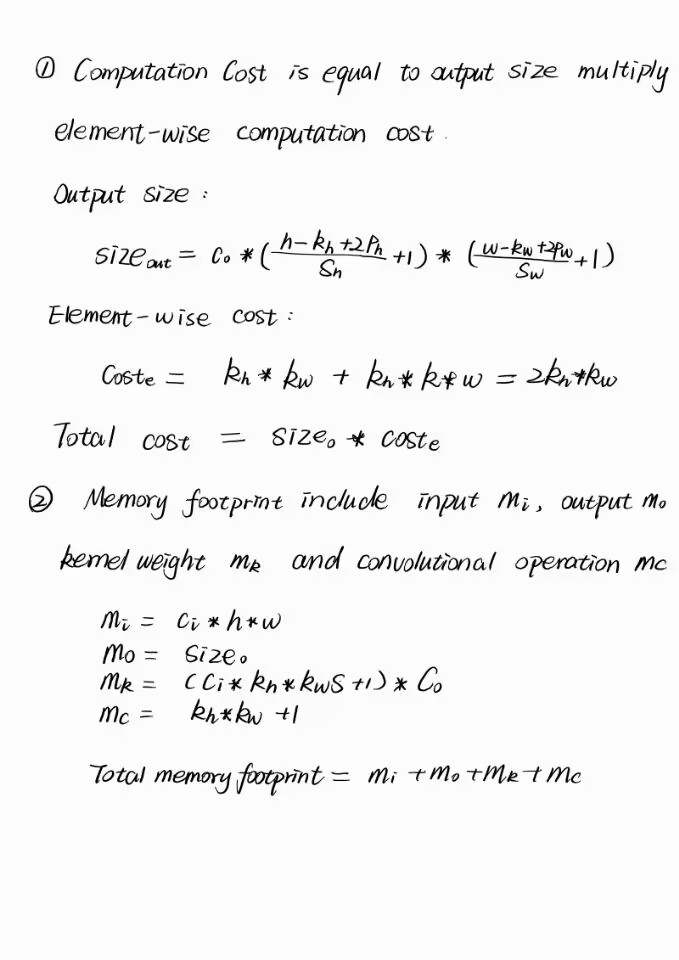
\includegraphics[scale=0.5]{1.jpg}
	\label{1}
\end{figure}


\newpage


\subsubsection*{2. Residual and Inception blocks (5 points)}
What are the major differences between the Inception block and the residual block? After removing some paths in the Inception block, how are they related to each other?

\textbf{Ans.} 
\begin{itemize}
	\item Inception block uses multiple paths while residual block uses one single path with X. 
	\item Thay can relate to others by adding a path connected each other like a residual block, may be there will need a 1x1 Conv.
\end{itemize}


\newpage


\subsubsection*{3. Optimization (5 points)}
Consider a simple multilayer perceptron with a single hidden layer of, say,  $d$  dimensions in the hidden layer and a single output. Show that for any local minimum there are at least  $d!$  equivalent solutions that behave identically.

\textbf{Ans.}If one permutes the connections of the hidden layer ($d!$ ways to do that), and move and rename connections appropriately, then one effectively has the same MLP with the exact same minima, yet the configuration has changed (in a trivial sense). Thus there are at least $d!$ configurations only trivialy different with the exact same minima.

As the network is a MLP the equation would be
$$O_{hidden}=\sum^d_{i=1}w_{\pi_i}\cdot x+b_{\pi_i}$$

$\pi_i$ is some order of the connections. For example $\pi_i = i$. And for $d$ items there are $d!$ permutations thus $d!$ order functions $\pi(i)=\pi_i$.

\end{document}